\clearpage% Flush earlier floats (otherwise order might not be correct)
\newpage


\section{Genetic algorithm}\label{sec:genetic-algorithm}
This section concludes the whole chapter by presenting the genetic algorithm
which is used to find an individual representing (sub)-optimal solution to the painting placement problem.
Pseudocode is presented in algorithm~\ref{alg:genetic}, initial population generation strategy is described in
subsection~\ref{subsec:initial-population}, and reproductive plan is described in subsection~\ref{subsec:reproductive-plan}.

Genetic algorithm has two main properties that have to be well-balanced with respect to each other
– diversification and intensification~\cite{blumMetaheuristicsCombinatorialOptimization2003}.\\

\navesti{Intensification} is the ability to identify parts of the search space with a high-quality
solutions.\\

\navesti{Diversification} is the ability to prevent premature convergence to the suboptimal solutions.\\

We can classify genetic operators in terms of their intensification and diversification effects.
The mutation operator is considered the most straightforward diversification strategy,
as it creates a small change in an individual's chromosome that can lead the search out of the suboptimal solution~\cite{blumMetaheuristicsCombinatorialOptimization2003}.
On the other hand, crossover creates a new solution by recombination of already present
individuals, which can be considered a diversification strategy~\cite{blumMetaheuristicsCombinatorialOptimization2003}.
However, researchers in~\cite{hanshengBalanceExplorationExploitation1999} argue that crossover
also has an intensification effect.
They argue that if the population were primarily composed of the same individuals, the crossover would not be able to improve the solution.
\\

\begin{algorithm}[H]
    \SetAlgoLined
    \LinesNumbered

    \SetKwData{Best}{best}
    \SetKwData{Candidate}{candidate}
    \SetKwData{Population}{population}
    \SetKwData{MaxNumberOfIter}{maxNumberOfIter}
    \SetKwData{Nil}{NIL}

    \SetKwFunction{Objective}{objective}
    \SetKwFunction{SelectBest}{selectBest}
    \SetKwFunction{GenerateInitialPopulation}{generateInitialPopulation}
    \SetKwFunction{ApplyReproductivePlan}{applyReproductivePlan}


    %%%%%%%%%%%%%%%%%%%%%%%%

    \Population $\leftarrow$ \GenerateInitialPopulation \\
    \Best $\leftarrow$ \SelectBest{\Population} \\

    \For{$i\leftarrow 1$ \KwTo \MaxNumberOfIter}{
        \Population $\leftarrow$ \ApplyReproductivePlan{\Population} \\
        \Candidate $\leftarrow$ \SelectBest{\Population} \\
        \If{\Objective{\Candidate} $<$ \Objective{\Best}}{
            \Best $\leftarrow$ \Candidate
        }
    }
    \KwRet{\Best}

    \caption{Genetic algorithm}\label{alg:genetic}
\end{algorithm}

\subsection{Initial population}\label{subsec:initial-population}
The initial population is the population that is used as a starting point for the genetic algorithm.
It consists of two parts – RANDOM and GREEDY.
Visualization can be seen on the left of the figure~\ref{fig:population-schema}.
\\

\navesti{RANDOM} part consists of randomly generated individuals.
The process of generating is (1) fill vectors $PS_{rk}$, $SO_{rk}$ and matrix $OR_{prob}$ with random values from $\langle 0,1 \rangle$,
and then (2) normalize $PS_{rk}, SO_{rk}$ and rows of $OR_{prob}$  to stochastic vectors to meet constraints in~\ref{eq:constraints}.\\

\navesti{GREEDY} part consists of individuals who are, at worst, as good as RANDOM.
The process of generating $k$ GREEDY individuals is (1) to create $100k$ RANDOM individuals and (2) to select $k$ best ones
in terms of their objective value.\\

Incorporating GREEDY individuals into the initial population may decreases the time the genetic algorithm needs to find a space with high-quality solutions.
The reason for adding RANDOM individuals is that greedy solutions might increase the chance
of an algorithm getting caught in local optima.

\begin{figure}[!h]
    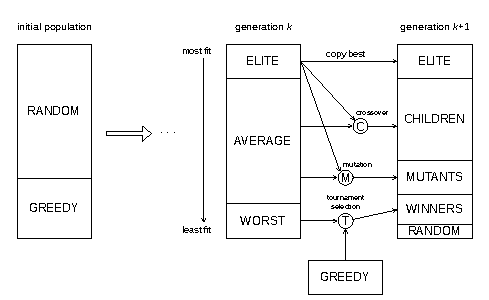
\includegraphics[width=1\textwidth, center]{pupulation_schema}
    \caption[Initial population generation strategy and transition]
    {Initial population generation strategy and transition from generation $k$ to $k+1$ using a reproductive plan.}
    \label{fig:population-schema}
\end{figure}


\newpage

\subsection{Reproductive plan}\label{subsec:reproductive-plan}
This section describes a reproductive plan used in this thesis.
It is visualized on the right of the figure~\ref{fig:population-schema}.
The reproductive plan starts with partitioning the individuals in the current
population into three groups according to their performance.\\

\navesti{ELITE} individuals are the ones that decode to the solutions with the lowest objective value.\\

\navesti{WORST} are the ones that decode to the solutions the highest objective value.\\

\navesti{AVERAGE} individuals are in between the ELITE and WORST.\\

Then, the elitism strategy is used.
It copies all ELITE individuals to the next generation.
Elitism enforces intensification, keeping the best individuals inside the population without any
modification or recombination with others.
It increases the representation of current (sub)-optimal solutions in the population, and thus it is
more likely that operators increasing intensification will use ELITE as an input.
In addition, without elitism, the best individuals might be lost after crossing over or mutation.

The next step is to use crossover and mutation genetic operators, with the crossover being
the most significant in terms of the individuals it produces for the next generation.\\

\navesti{CHILDREN} are individuals that are created using a crossover, with the first parent being selected
at random from ELITE and the second parent selected at random from AVERAGE.\\

\navesti{MUTANTS} are individuals that are created using a mutation,
with an input selected at random from ELITE and AVERAGE.\\

Another step is the tournament selection between the least performant and greedily generated individuals.
Reason for it is that the least performant individuals often receive high penalization
values in objective~\ref{eq:objective}.
It means that they produce solutions with mostly overlapping paintings.
\\

\navesti{WINNER} individuals result from tournament selection between WORST and GREEDY.
Selection picks the best individuals from WORST and GREEDY until all available spots for WINNER are filled. \\

Finally, RANDOM, a small group of randomly generated individuals, is injected into the next population.
The reason is to decrease the chance of the genetic algorithm getting stuck in a local optimum
by randomly adding samples from the search space.
